\part{La construction}
\label{part:construction}

\chapter{Les images des machines louées}
\label{chap:images}

\section{Le problème : plusieurs services dans un conteneur}

Un conteneur exécute \emph{un} processus. Quand ce processus se termine, le
conteneur s'arrête. C'est voulu : un conteneur est censé faire une chose.

Or une machine louée doit en faire plusieurs à la fois : un serveur SSH, un
terminal web, et en mode bureau un serveur d'affichage, un gestionnaire de
fenêtres et une passerelle VNC vers le navigateur. Cinq processus.

Il faut donc un \emph{superviseur} : un processus qui démarre les autres, les
surveille, et relance celui qui meurt. Nous utilisons \cmd{supervisord}.

\begin{notion}{PID 1 et la responsabilité d'\emph{init}}
Le premier processus d'un espace de noms PID porte le numéro 1 et hérite d'une
obligation : adopter les processus orphelins et récupérer leur code de sortie.
Sans cela, les processus terminés s'accumulent à l'état \emph{zombie}.

Un \cmd{bash} lancé comme PID 1 ne fait pas ce travail. \cmd{supervisord}, si.
\end{notion}

\section{Trois Dockerfiles, six images}

Le projet propose trois distributions en deux modes. Plutôt que six fichiers,
on en écrit trois --- un par distribution --- et le mode devient un paramètre
de construction.

\begin{lstlisting}[language=dockerfile,caption={\fichier{1\_docker/Dockerfile} --- la structure (extraits)}]
FROM ubuntu:22.04

# DESKTOP=1 ajoute le serveur d'affichage, XFCE et noVNC.
ARG DESKTOP=0

RUN apt-get update \
    && apt-get install -y --no-install-recommends \
         openssh-server supervisor ca-certificates \
    && rm -rf /var/lib/apt/lists/*

# ... installation conditionnelle du bureau selon DESKTOP ...

COPY entrypoint.sh /usr/local/bin/entrypoint.sh
RUN chmod +x /usr/local/bin/entrypoint.sh

EXPOSE 22 7681 6080
CMD ["/usr/local/bin/entrypoint.sh"]
\end{lstlisting}

\begin{piege}{\texttt{apt-get install} sans nettoyage dans le même \texttt{RUN}}
Chaque instruction \cmd{RUN} crée une couche. Si l'on installe des paquets
dans une couche et qu'on efface le cache d'apt dans la couche
\emph{suivante}, le cache reste présent dans l'image : une couche ne peut pas
alléger celle du dessous.

Il faut donc enchaîner installation et nettoyage dans \emph{le même}
\cmd{RUN}, comme ci-dessus. Sur nos images, cela représente une cinquantaine
de mégaoctets.
\end{piege}

\begin{piege}{Un mot de passe par défaut dans l'image}
Notre première version contenait \cmd{ENV ROOT\_PASSWORD=insacloud}.
L'analyseur \cmd{hadolint} l'a signalé (règle DL3064), et il avait raison : ce
mot de passe aurait été le même sur \emph{toutes} les machines louées, et
visible par quiconque fait \cmd{docker history} sur l'image.

La correction : aucun mot de passe dans l'image. Si la plateforme n'en fournit
pas, l'entrypoint en tire un au hasard.
\end{piege}

\section{Le script de démarrage}

\begin{lstlisting}[language=bash,caption={\fichier{1\_docker/entrypoint.sh} --- le repli sûr}]
# Mot de passe root : fourni par la plateforme (-e ROOT_PASSWORD=...). S'il
# manque, on en tire un au hasard plutot que de retomber sur une valeur connue :
# un mot de passe par defaut serait le meme sur toutes les machines louees.
if [ -z "${ROOT_PASSWORD:-}" ]; then
    ROOT_PASSWORD="$(tr -dc 'A-Za-z2-9' < /dev/urandom | head -c 16)"
    echo "[insacloud] Aucun ROOT_PASSWORD fourni : tire au hasard = ${ROOT_PASSWORD}"
fi
\end{lstlisting}

Le script écrit ensuite une configuration \cmd{supervisord} adaptée au mode,
puis se remplace par le superviseur :

\begin{lstlisting}[language=bash]
exec "$(command -v supervisord)" -c "$CONF"
\end{lstlisting}

\begin{notion}{Pourquoi \texttt{exec}}
Sans \cmd{exec}, le shell resterait PID 1 et lancerait supervisord comme
enfant. Les signaux envoyés par Docker (\cmd{docker stop}) iraient au shell,
qui ne les relaierait pas : l'arrêt deviendrait brutal au bout du délai de
grâce.

\cmd{exec} remplace le processus courant : supervisord \emph{devient} le PID 1
et reçoit les signaux directement.
\end{notion}

\begin{figure}[htbp]
\centering
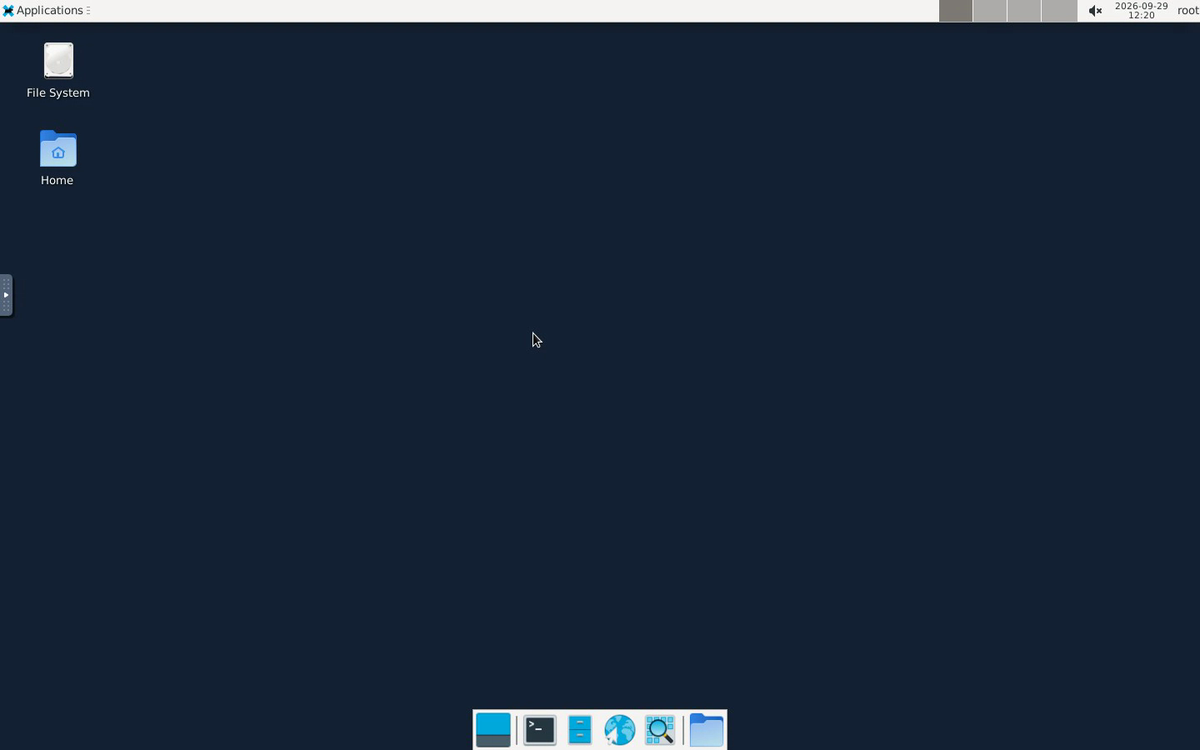
\includegraphics[width=0.78\textwidth]{../docs/08-bureau-xfce.png}
\caption{Le mode « bureau » : cinq processus cohabitent dans le conteneur ---
sshd, le terminal web, le serveur d'affichage, XFCE et la passerelle noVNC ---
tous surveillés par supervisord.}
\end{figure}

\section{Rotation du mot de passe à chaud}

L'utilisateur peut régénérer le mot de passe de sa machine sans la redémarrer.
Le même script sert de point d'entrée et d'outil :

\begin{lstlisting}[language=bash]
docker exec <conteneur> /usr/local/bin/entrypoint.sh setpass <nouveau>
\end{lstlisting}

SSH, terminal web et bureau prennent le nouveau mot de passe immédiatement.

\chapter{Piloter Docker depuis Python}

\section{Pourquoi la ligne de commande et pas un SDK}

Il existe une bibliothèque Python officielle (\cmd{docker-py}). Le cahier des
charges impose pourtant une commande précise :

\begin{center}
\cmd{docker run -d --restart=always -p <port>:22 <image>}
\end{center}

Piloter la CLI par \cmd{subprocess} rend cette commande \emph{visible dans le
code}. Chaque option passée se lit telle quelle. C'est un choix de lisibilité
et de conformité, pas une facilité.

\begin{lstlisting}[language=Python,caption={\fichier{2\_webapp/docker\_ops.py} --- l'appel central}]
def run_docker(*args, worker: str = "local", timeout: int = DOCKER_TIMEOUT) -> str:
    """Execute `docker <args>` sur le noeud `worker` (local ou distant via SSH)."""
    cmd = [*wk.docker_command(worker), *args]
    try:
        # Appel sans shell : les arguments sont passes en liste, donc jamais
        # re-interpretes par un interpreteur de commandes. Les seules valeurs
        # d'origine utilisateur (duree, distribution, mode) sont validees en amont.
        res = subprocess.run(cmd, capture_output=True, text=True, timeout=timeout)
    except FileNotFoundError as erreur:
        raise DockerError("La commande 'docker' est introuvable sur le serveur.") from erreur
    except subprocess.TimeoutExpired as erreur:
        raise DockerError("Docker n'a pas repondu dans le delai imparti.") from erreur
    if res.returncode != 0:
        message = res.stderr.strip() or f"docker {args[0]} a echoue ({res.returncode})"
        raise DockerError(message)
    return res.stdout.strip()
\end{lstlisting}

\begin{piege}{\texttt{shell=True} est une porte ouverte}
Écrire \cmd{subprocess.run(f"docker run ... \{nom\}", shell=True)} laisserait un
utilisateur nommer sa machine \cmd{x; rm -rf /} et faire exécuter n'importe
quoi au serveur. C'est une \emph{injection de commande}.

Passer une \textbf{liste} d'arguments, sans \cmd{shell}, supprime le problème
à la racine : il n'y a aucun interpréteur pour relire la chaîne. Chaque
élément de la liste est un argument, point.
\end{piege}

\section{La création d'une machine}

\begin{lstlisting}[language=Python,caption={\fichier{2\_webapp/docker\_ops.py} --- la commande imposée, complétée}]
def docker_run_container(port, name, root_password, os_type, mode,
                         term_port, gui_port=None, ssh_public_key=None,
                         worker="local") -> str:
    spec = MODES[mode]
    args = [
        "run", "-d",
        "--restart=always",
        "-p", f"{port}:22",
        "-p", f"{term_port}:{TERM_CONTAINER_PORT}",
        "--name", name,
        "-e", f"ROOT_PASSWORD={root_password}",
        *CONTAINER_HARDENING,
    ]
    if ssh_public_key:
        args += ["-e", f"SSH_PUBKEY={ssh_public_key}"]
    if spec["gui"] and gui_port:
        args += ["-p", f"{gui_port}:{GUI_CONTAINER_PORT}", "--shm-size", "512m"]
    if spec["memory"]:
        # Le cours impose de definir reservation ET limite : la reservation est
        # le minimum garanti en cas de contention, la limite le plafond dur.
        args += ["--memory", spec["memory"],
                 "--memory-reservation", spec["reservation"]]
    args.append(image_for(os_type, mode))
    return run_docker(*args, worker=worker)[:12]
\end{lstlisting}

\section{Le durcissement, option par option}

\begin{lstlisting}[language=Python]
CONTAINER_HARDENING = [
    "--label", f"{MACHINE_LABEL}={MACHINE_LABEL_VALUE}",
    "--label", f"{CLUSTER_LABEL}={CLUSTER}",
    "--cap-drop", "ALL",
    "--cap-add", "CHOWN", "--cap-add", "DAC_OVERRIDE", "--cap-add", "FOWNER",
    "--cap-add", "FSETID", "--cap-add", "SETGID", "--cap-add", "SETUID",
    "--cap-add", "SYS_CHROOT", "--cap-add", "NET_BIND_SERVICE",
    "--cap-add", "KILL", "--cap-add", "AUDIT_WRITE",
    "--security-opt", "no-new-privileges:true",
    "--pids-limit", CONTAINER_PIDS_LIMIT,
    "--cpus", CONTAINER_CPUS,
]
\end{lstlisting}

\begin{center}
\small
\begin{tabularx}{\textwidth}{@{}lX@{}}
\toprule
\textbf{Option} & \textbf{Ce qu'elle empêche} \\
\midrule
\cmd{--cap-drop ALL} & tout pouvoir de root, avant d'en rendre dix \\
\cmd{--cap-add NET\_BIND\_SERVICE} & sans elle, sshd ne peut pas écouter sur le port 22 \\
\cmd{no-new-privileges} & qu'un binaire \emph{setuid} regagne des droits \\
\cmd{--pids-limit} & une \emph{fork bomb} qui sature la table des processus \\
\cmd{--cpus} & qu'un minage monopolise les cœurs du nœud \\
\cmd{--memory} & qu'une fuite mémoire fasse tomber les voisins \\
\bottomrule
\end{tabularx}
\end{center}

\section{Reconnaître ses machines : l'erreur qui a tout détruit}

Le Faucheur doit savoir quels conteneurs lui appartiennent. Notre première
version les reconnaissait à leur nom, qui commence par \cmd{insacloud\_}.

Puis nous avons déployé la pile \cmd{docker compose}, dont les conteneurs
s'appellent \cmd{insacloud-web}, \cmd{insacloud-db}, \cmd{insacloud-faucheur}.
Le Faucheur les a pris pour des machines louées orphelines et les a détruits.
\textbf{Il s'est supprimé lui-même.}

\begin{lstlisting}[language=Python,caption={\fichier{2\_webapp/docker\_ops.py} --- l'identité par étiquette}]
# Label appose a TOUTE machine louee. C'est lui, et non le nom du conteneur,
# qui identifie ce que la plateforme a le droit de detruire : un prefixe de nom
# est trop facile a percuter.
MACHINE_LABEL = "insacloud.role"
MACHINE_LABEL_VALUE = "rented-machine"
CLUSTER_LABEL = "insacloud.cluster"

# Les deux filtres sont combines : une machine doit etre une machine louee ET
# appartenir a CE deploiement. Sans le second, le Faucheur d'une plateforme
# detruirait les machines d'une autre tournant sur le meme demon.
MACHINE_FILTERS = [f"label={MACHINE_LABEL}={MACHINE_LABEL_VALUE}",
                   f"label={CLUSTER_LABEL}={CLUSTER}"]
\end{lstlisting}

\begin{retenir}
Un nom est une commodité d'affichage ; une étiquette est une identité. Dès
qu'un programme doit décider de \emph{détruire} quelque chose, il doit se
fonder sur une marque qu'il a lui-même apposée, jamais sur une convention de
nommage.
\end{retenir}

Le second label a été ajouté après un deuxième incident : deux déploiements
partageant un même démon Docker se détruisaient mutuellement leurs conteneurs.

\chapter{La base de données}
\label{chap:bdd}

\section{SQLAlchemy : pourquoi un ORM}

On peut écrire du SQL à la main. On s'expose alors à trois choses : les
injections SQL si l'on concatène des chaînes, l'incompatibilité entre SQLite et
PostgreSQL, et l'absence de vérification à l'écriture.

Un \emph{ORM} (\emph{Object-Relational Mapper}) fait correspondre une classe
Python à une table. On écrit des objets, il écrit le SQL --- toujours avec des
paramètres liés, donc sans injection possible.

\begin{lstlisting}[language=Python,caption={\fichier{2\_webapp/models.py} --- une table}]
class Rental(Base):
    __tablename__ = "rentals"

    id: Mapped[int] = mapped_column(Integer, primary_key=True)
    user_id: Mapped[int] = mapped_column(ForeignKey("users.id"), nullable=False)
    instance_id: Mapped[int] = mapped_column(ForeignKey("instances.id"), nullable=False)
    start_time: Mapped[datetime] = mapped_column(DateTime, default=utc_now, nullable=False)
    end_time: Mapped[datetime] = mapped_column(DateTime, nullable=False)
    status: Mapped[str] = mapped_column(String(16), default=RENTAL_ACTIVE, nullable=False)

    user: Mapped["User"] = relationship(back_populates="rentals")
    instance: Mapped["Instance"] = relationship(back_populates="rental")

    __table_args__ = (Index("idx_rentals_end", "status", "end_time"),)
\end{lstlisting}

\begin{notion}{Clé étrangère}
\cmd{ForeignKey("users.id")} déclare que cette colonne pointe vers la table
\texttt{users}. La base refusera alors une location dont l'utilisateur n'existe
pas : la cohérence est garantie par le moteur, pas par la discipline du
développeur.
\end{notion}

\section{Alembic : faire évoluer un schéma sans perdre les données}

Tant qu'on développe, on efface la base et on recommence. Dès qu'il y a des
données réelles, c'est impossible : il faut \emph{migrer}.

Alembic enregistre chaque changement de schéma dans un fichier numéroté, et
chaque fichier connaît son prédécesseur. La base retient où elle en est.

\begin{lstlisting}[language=bash]
# Comparer les modeles a la base et generer la migration correspondante
alembic revision --autogenerate -m "archives du travail des utilisateurs"

# Appliquer tout ce qui manque
alembic upgrade head

# Verifier que la base correspond aux modeles (utilise par la CI)
alembic check
\end{lstlisting}

\begin{piege}{SQLite ne sait pas modifier une colonne}
PostgreSQL accepte \cmd{ALTER TABLE ... ALTER COLUMN}. SQLite, non : il faut
créer une table neuve, recopier, supprimer l'ancienne, renommer.

Alembic sait le faire, mais seulement si on le lui demande avec
\cmd{render\_as\_batch=True}. Sans cette option, les migrations passent en
développement sur PostgreSQL et échouent sur le SQLite d'un poste --- ou
l'inverse.
\end{piege}

\section{La course au démarrage : un bug qui ne se voit qu'en production}

Gunicorn lance quatre processus. Chacun importe l'application, qui appelle
\cmd{init\_db()}, qui crée les tables si elles manquent. Les quatre le font
\emph{en même temps}.

Le résultat est intermittent : parfois tout se passe bien, parfois un processus
meurt avec \cmd{table users already exists}. Sur un poste de développement
mono-processus, le bug n'apparaît jamais.

\begin{lstlisting}[language=Python,caption={\fichier{2\_webapp/database.py} --- création tolérante à la concurrence}]
for tentative in range(5):
    try:
        Base.metadata.create_all(engine)
        break
    except (OperationalError, ProgrammingError) as erreur:
        message = str(erreur).lower()
        if "already exists" in message:
            # Un autre processus a cree le schema entre notre verification et
            # notre creation : c'est exactement le resultat voulu.
            log.info("Schema cree simultanement par un autre processus.")
            break
        if "locked" not in message or tentative == 4:
            raise
        time.sleep(0.3 * (tentative + 1))
\end{lstlisting}

Nous avons reproduit la panne en lançant huit processus simultanés : six sur
huit démarraient. Après correction, huit sur huit. La chaîne d'intégration
lance désormais Gunicorn avec \cmd{--preload}, qui importe l'application
\emph{une fois} avant de dupliquer le processus.

\begin{retenir}
Un bug de concurrence ne se trouve pas en relisant le code : il se trouve en
lançant plusieurs processus à la fois et en recommençant. Si vous ne savez pas
reproduire un bug, vous ne saurez pas vérifier qu'il est corrigé.
\end{retenir}

\section{Ne jamais journaliser un secret}

Le Faucheur affichait au démarrage l'URL de la base --- qui contient le mot de
passe PostgreSQL --- en clair dans \cmd{journalctl}. Trouvé en lisant nos
propres journaux. Toute URL passe désormais par une fonction de masquage avant
d'être écrite.

\begin{lstlisting}[language=Python,caption={\fichier{2\_webapp/database.py}}]
def url_sans_secret(url: str) -> str:
    """Masque le mot de passe d'une URL de connexion avant de la journaliser."""
\end{lstlisting}

\chapter{L'application et son API}

\section{Une organisation en couches}

\begin{center}
\small
\begin{tabularx}{\textwidth}{@{}lX@{}}
\toprule
\textbf{Fichier} & \textbf{Responsabilité} \\
\midrule
\fichier{app.py} & les routes HTML, les sessions, les en-têtes de sécurité \\
\fichier{api.py} & les routes JSON du cahier des charges \\
\fichier{services.py} & la logique métier : louer, arrêter, prolonger, reprendre \\
\fichier{database.py} & tous les accès à la base \\
\fichier{docker\_ops.py} & tout ce qui parle à Docker \\
\fichier{models.py} & la description des tables \\
\fichier{crypto.py} & les clés et le chiffrement \\
\fichier{workers.py} & la résolution des nœuds et le choix du moins chargé \\
\bottomrule
\end{tabularx}
\end{center}

La règle qui tient l'ensemble : \textbf{les couches basses ne connaissent pas
les hautes}. \fichier{docker\_ops.py} ignore l'existence de Flask et de la
base. On peut donc le tester sans serveur, et le Faucheur peut l'utiliser
directement.

\section{Le résultat d'une opération}

Plutôt que de renvoyer des exceptions ou des tuples, les services renvoient un
objet uniforme :

\begin{lstlisting}[language=Python,caption={\fichier{2\_webapp/services.py}}]
@dataclass
class Resultat:
    ok: bool
    message: str
    code: int = 200
    donnees: dict = field(default_factory=dict)
\end{lstlisting}

La route HTML en tire un message \cmd{flash} et une redirection ; la route
JSON en tire un corps et un code HTTP. La logique métier, elle, ne sait pas
laquelle des deux l'appelle.

\section{Les points d'entrée imposés}

Le cahier des charges fixe un contrat d'API précis. Les voici, tels
qu'implémentés :

\begin{center}
\small
\begin{tabularx}{\textwidth}{@{}llX@{}}
\toprule
\textbf{Méthode} & \textbf{Chemin} & \textbf{Rôle} \\
\midrule
GET & \cmd{/health} & état du service, de la base et du parc \\
GET & \cmd{/distributions} & le catalogue des systèmes disponibles \\
GET & \cmd{/instances} & les machines de l'utilisateur connecté \\
GET & \cmd{/instances/\{id\}} & le détail d'une machine \\
POST & \cmd{/rent} & louer une machine \\
POST & \cmd{/instances/\{id\}/stop} & arrêter et détruire \\
POST & \cmd{/instances/\{id\}/extend} & prolonger la location \\
GET & \cmd{/workers} & l'état du parc \\
GET & \cmd{/workers/\{id\}} & le détail d'un nœud \\
POST & \cmd{/workers/register} & inscription d'un agent \\
POST & \cmd{/workers/heartbeat} & battement de cœur d'un agent \\
\bottomrule
\end{tabularx}
\end{center}

\begin{lstlisting}[language=bash,caption={Louer une machine en JSON}]
curl -s -c biscuits -b biscuits -H 'Content-Type: application/json' \
     -d '{"username":"aziz","password":"..."}' http://127.0.0.1:8088/login

curl -s -c biscuits -b biscuits -H 'Content-Type: application/json' \
     -d '{"distribution":"alpine","mode":"terminal","duration":30}' \
     http://127.0.0.1:8088/rent | jq
\end{lstlisting}

\begin{notion}{Pourquoi \texttt{/health} compte}
Une sonde d'état permet à un orchestrateur, à un équilibreur de charge ou à
une chaîne de déploiement de savoir si le service est réellement utilisable.
Ici, elle vérifie aussi la base et le parc : un service qui répond mais dont
la base est injoignable n'est pas en bonne santé.

La chaîne d'intégration s'en sert comme preuve finale : un déploiement qui ne
sert pas fait échouer la chaîne.
\end{notion}

\section{Protéger les routes des agents}

Les agents ne sont pas des utilisateurs : ils n'ont pas de session. Ils
s'authentifient par un jeton partagé, dans un en-tête.

\begin{lstlisting}[language=Python,caption={\fichier{2\_webapp/api.py} --- comparaison en temps constant}]
def token_agent_requis(vue):
    @functools.wraps(vue)
    def enveloppe(*args, **kwargs):
        presente = request.headers.get("X-Agent-Token", "")
        # compare_digest : la duree de la comparaison ne depend pas du nombre
        # de caracteres corrects. Un « == » permettrait de deviner le jeton
        # caractere par caractere en mesurant le temps de reponse.
        if not AGENT_TOKEN or not hmac.compare_digest(presente, AGENT_TOKEN):
            return jsonify(error="Jeton d'agent invalide."), 401
        return vue(*args, **kwargs)
    return enveloppe
\end{lstlisting}

\begin{notion}{Attaque temporelle}
L'opérateur \cmd{==} sur deux chaînes s'arrête au premier caractère différent.
En mesurant très précisément le temps de réponse, un attaquant peut découvrir
le secret caractère par caractère. \cmd{hmac.compare\_digest} compare toujours
l'intégralité, en temps constant.
\end{notion}

\chapter{Le parc de nœuds}

\section{L'agent, en bibliothèque standard seulement}

L'agent tourne sur chaque worker. Il pourrait utiliser \cmd{requests}, mais
cela imposerait d'installer des dépendances Python sur chaque nœud. Il n'emploie
donc que la bibliothèque standard : \cmd{urllib} pour les appels,
\cmd{/proc/meminfo} pour la mémoire, \cmd{os.cpu\_count()} pour les cœurs.

\begin{lstlisting}[language=Python,caption={\fichier{2\_webapp/worker\_agent.py} --- se présenter}]
def enregistrer() -> bool:
    """Presente le noeud au controleur. Retourne True si l'inscription a pris."""
    charge = {
        "hostname": nom_du_noeud(),
        "ip": adresse_du_noeud(),
        "cpu": nombre_de_coeurs(),
        "memory": memoire_totale_mio(),
        "docker": docker_operationnel(),
    }
    code, corps = appeler("/workers/register", charge)
    if code in (200, 201):
        log.info("Enregistre aupres de %s : %s (%s coeurs, %s Mio, capacite %s)",
                 CONTROLLER, charge["hostname"], charge["cpu"], charge["memory"],
                 corps.get("capacity"))
        return True
    log.error("Enregistrement refuse (%s) : %s", code, corps.get("error", corps))
    return False
\end{lstlisting}

\section{Le battement de cœur, et les trois états}

\begin{lstlisting}[language=Python,caption={\fichier{2\_webapp/worker\_agent.py} --- signaler sa présence}]
def battre() -> bool:
    """
    Envoie un battement de coeur. Annonce BUSY si le noeud est sature, pour que
    l'ordonnanceur cesse d'y envoyer des machines sans le declarer en panne.
    """
    if not docker_operationnel():
        log.warning("Docker ne repond pas : aucun battement envoye.")
        return False
    charge = {"hostname": nom_du_noeud(), "containers": conteneurs_actifs()}
    code, corps = appeler("/workers/heartbeat", charge)
    if code == 200:
        return True
    if code == 404 and corps.get("action") == "register":
        log.warning("Noeud inconnu du controleur : nouvelle inscription.")
        return enregistrer()
    return False
\end{lstlisting}

\begin{center}
\small
\begin{tabularx}{\textwidth}{@{}lX@{}}
\toprule
\textbf{État} & \textbf{Signification} \\
\midrule
\cmd{AVAILABLE} & le nœud bat, Docker répond, il reste de la place \\
\cmd{BUSY} & le nœud bat, mais il a atteint sa capacité : on ne lui envoie plus rien \\
\cmd{OFFLINE} & plus de battement depuis 90 s : ses machines sont recréées ailleurs \\
\bottomrule
\end{tabularx}
\end{center}

\begin{retenir}
La distinction \cmd{BUSY} / \cmd{OFFLINE} est essentielle. Un nœud saturé est
en bonne santé : il ne faut surtout pas détruire et recréer ses machines
ailleurs. Confondre « plein » et « mort » déclencherait des migrations
inutiles et coûteuses.
\end{retenir}

\section{Démarrer avant le contrôleur}

Au démarrage d'un cluster, les workers peuvent être prêts avant le contrôleur.
L'agent ne doit alors ni abandonner, ni marteler le réseau.

\begin{lstlisting}[language=Python]
    # L'inscription est retentee jusqu'a ce qu'elle passe : au demarrage d'un
    # cluster, le worker peut etre pret avant le controleur.
    attente = 5
    while not _arret.is_set() and not enregistrer():
        log.info("Nouvelle tentative dans %s s.", attente)
        _arret.wait(attente)
        attente = min(attente * 2, 60)
\end{lstlisting}

\begin{notion}{Recul exponentiel (\emph{exponential backoff})}
On double le délai à chaque échec, jusqu'à un plafond. Un service qui
retenterait toutes les secondes ajouterait sa charge à celle d'un contrôleur
déjà en difficulté. Doubler l'attente laisse au système le temps de se
rétablir.
\end{notion}

\section{L'ordonnanceur}

Le choix du nœud suit deux règles simples et une exclusion :

\begin{enumerate}
\item n'envisager que les nœuds \cmd{AVAILABLE} --- ni saturés, ni muets ;
\item parmi eux, prendre celui qui héberge le moins de machines ;
\item en cas d'égalité, le premier par ordre alphabétique, pour que le
  comportement soit reproductible et donc testable.
\end{enumerate}

\begin{retenir}
Un ordonnanceur déterministe est un ordonnanceur qu'on peut tester. Si le
départage en cas d'égalité est aléatoire, le test devient intermittent --- et
un test intermittent finit toujours par être ignoré.
\end{retenir}

\chapter{Le Faucheur}
\label{chap:faucheur}

\section{Un démon, trois missions}

Le Faucheur est un processus séparé de l'application. Il tourne en boucle,
toutes les dix secondes.

\begin{description}
\item[Expirer] détruire les machines dont la location est échue.
\item[Réconcilier] remettre Docker et la base d'accord.
\item[Surveiller le parc] déclarer hors ligne les nœuds muets et faire
  recréer leurs machines.
\end{description}

\begin{notion}{Pourquoi un processus séparé}
On pourrait lancer un fil d'exécution dans l'application. Mauvaise idée :
Gunicorn lance quatre processus, donc quatre Faucheurs qui se marcheraient
dessus. Un service distinct, démarré une seule fois par systemd, évite le
problème et peut être redémarré sans couper le site.
\end{notion}

\section{La réconciliation, ou l'art de douter de soi}

La base dit ce qui \emph{devrait} exister ; Docker dit ce qui existe
\emph{vraiment}. Les deux divergent : un conteneur tué à la main, un processus
interrompu au mauvais moment, un nœud redémarré.

\begin{lstlisting}[language=Python,caption={\fichier{2\_webapp/faucheur.py}}]
def reconcile() -> None:
    """
    Remet Docker et la BDD en coherence, noeud par noeud :
      - conteneur insacloud_* sans instance 'running' en BDD  -> docker rm -f
      - instance 'running' en BDD sans conteneur dans Docker  -> status 'stopped'
    Un noeud injoignable est simplement ignore (rien n'est modifie pour lui).
    """
\end{lstlisting}

\begin{piege}{Un nœud injoignable n'est pas un nœud vide}
C'est le piège le plus dangereux de la réconciliation. Si le nœud ne répond
pas, \cmd{docker ps} renvoie une liste vide. Un code naïf en conclurait que
toutes ses machines ont disparu et les marquerait « arrêtées » --- alors
qu'elles tournent parfaitement.

D'où la règle : un nœud injoignable est \emph{ignoré}, jamais interprété.
\end{piege}

\section{L'erreur du \texttt{+-1 minutes}}

Prolonger une location ajoute des minutes ; l'écourter en retire. Le code
construisait l'intervalle ainsi :

\begin{lstlisting}[language=Python]
f"+{int(minutes)} minutes"      # avec minutes = -1 : "+-1 minutes"
\end{lstlisting}

SQLite rejette \cmd{+-1 minutes}. Il faut demander explicitement le signe :

\begin{lstlisting}[language=Python]
f"{int(duration_minutes):+d} minutes"   # donne "+30 minutes" ou "-1 minutes"
\end{lstlisting}

\begin{notion}{Le format \texttt{:+d}}
En Python, \cmd{f"\{x:+d\}"} affiche toujours le signe : \cmd{+30} ou \cmd{-1}.
C'est exactement ce qu'attend la syntaxe des intervalles SQL.
\end{notion}

\chapter{La sécurité}
\label{chap:securite}

\section{Deux clés, jamais la même}

\begin{lstlisting}[language=Python,caption={\fichier{2\_webapp/crypto.py}}]
"""
Deux cles distinctes, jamais la meme :
  * la cle de session Flask, qui signe les cookies ;
  * la cle du coffre (Fernet), qui chiffre les mots de passe root en base.

Chacune vient de l'environnement — Ansible les injecte depuis son Vault — ou,
a defaut, d'un fichier local en 0600 cree une seule fois. Separer les deux
garantit qu'un vol de la cle de session ne donne pas acces aux machines louees.
"""
\end{lstlisting}

\begin{notion}{Fernet}
Fernet est une recette de chiffrement symétrique authentifié fournie par la
bibliothèque \cmd{cryptography}. Elle combine AES en mode CBC et un HMAC : on
ne peut ni lire le contenu sans la clé, ni le modifier sans que cela se voie.

Son intérêt pour un débutant : il n'y a aucun paramètre à choisir, donc aucune
occasion de se tromper de mode ou de vecteur d'initialisation.
\end{notion}

\section{Le mot de passe root : montré une fois, conservé chiffré}

\begin{enumerate}
\item À la création, 16 caractères sont tirés au sort (environ 90 bits
  d'entropie).
\item Ils sont affichés \emph{une seule fois} à l'utilisateur.
\item Ils sont chiffrés avec Fernet avant d'être écrits en base.
\item Pour les revoir, l'utilisateur ressaisit le mot de passe de \emph{son
  compte} : le coffre s'ouvre cinq minutes, puis se reverrouille.
\end{enumerate}

\begin{figure}[htbp]
\centering
\begin{minipage}{0.48\textwidth}
  \centering
  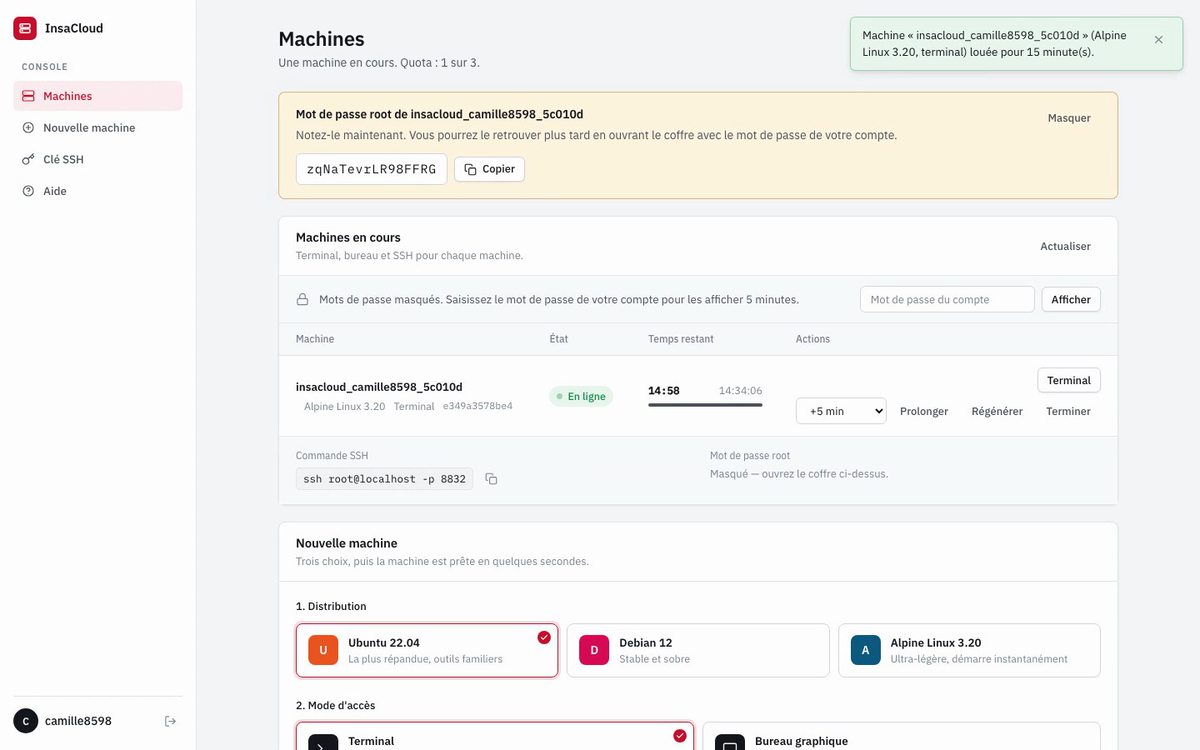
\includegraphics[width=\textwidth]{../docs/05-mot-de-passe-unique.png}
\end{minipage}\hfill
\begin{minipage}{0.48\textwidth}
  \centering
  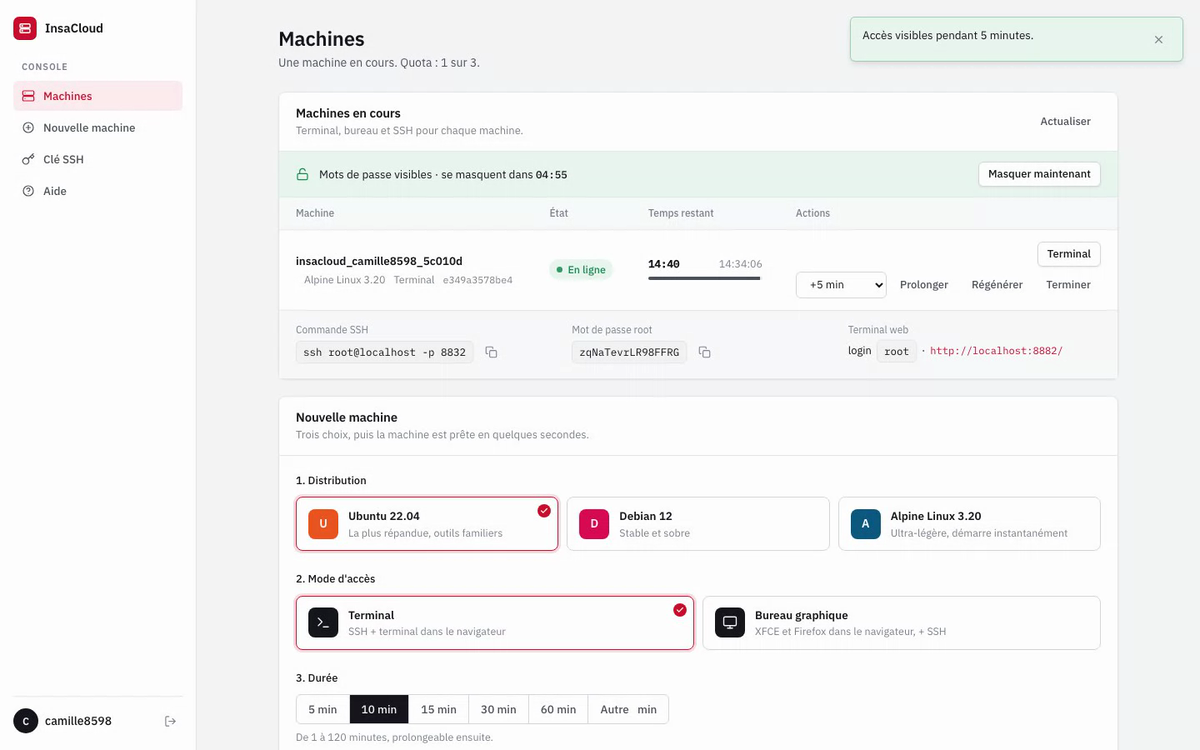
\includegraphics[width=\textwidth]{../docs/06-coffre-ouvert.png}
\end{minipage}
\caption{À gauche, l'affichage unique à la création. À droite, le coffre
rouvert après re-authentification : les accès redeviennent visibles cinq
minutes.}
\end{figure}

\begin{lstlisting}[language=Python,caption={\fichier{2\_webapp/app.py} --- plus rien de secret dans le cookie}]
def reveal_secret(instance_id: int, rotated: bool = False) -> None:
    # On ne depose que l'IDENTIFIANT de la machine dans la session. Le secret
    # lui-meme est relu en base, dechiffre, au moment de l'affichage.
    session["reveal"] = {"instance": int(instance_id), "rotated": bool(rotated)}

def secret_a_reveler():
    marqueur = session.pop("reveal", None)
    if not marqueur or g.user is None:
        return None
    # Le proprietaire est verifie dans la requete : l'identifiant d'une machine
    # d'autrui ne donne rien, meme si la session etait forgee.
    instance = db.get_instance(marqueur.get("instance"), user_id=g.user["id"])
    if instance is None or instance["status"] != db.STATUS_RUNNING:
        return None
    secret = decrypt_secret(instance["root_password"])
\end{lstlisting}

\section{CSRF : empêcher un autre site d'agir en votre nom}

\begin{notion}{\emph{Cross-Site Request Forgery}}
Vous êtes connecté à notre plateforme. Vous visitez un site malveillant qui
contient un formulaire invisible pointant vers \cmd{/instances/3/stop}, soumis
automatiquement. Votre navigateur joint vos cookies : la requête est
authentifiée, et votre machine s'arrête.

La parade : un jeton imprévisible, déposé dans la session et recopié dans
chaque formulaire. Le site malveillant ne peut pas le deviner --- il ne peut
pas lire votre session.
\end{notion}

\begin{piege}{Exempter les requêtes JSON, mais pourquoi ?}
L'API doit pouvoir être appelée par \cmd{curl}, qui n'a pas de jeton. Notre
exemption porte sur \cmd{Content-Type: application/json}, et elle est sûre pour
deux raisons :
\begin{itemize}
\item un formulaire HTML ne peut \emph{pas} émettre ce type de contenu --- il
  est limité à trois types, dont aucun n'est JSON ;
\item une requête \cmd{fetch} qui le fait depuis un autre site déclenche une
  vérification \emph{preflight} CORS, que le serveur refuse.
\end{itemize}
Le raisonnement compte autant que la règle : exempter sans comprendre ouvrirait
exactement le trou qu'on cherche à boucher.
\end{piege}

\begin{figure}[htbp]
\centering
\begin{minipage}{0.48\textwidth}
  \centering
  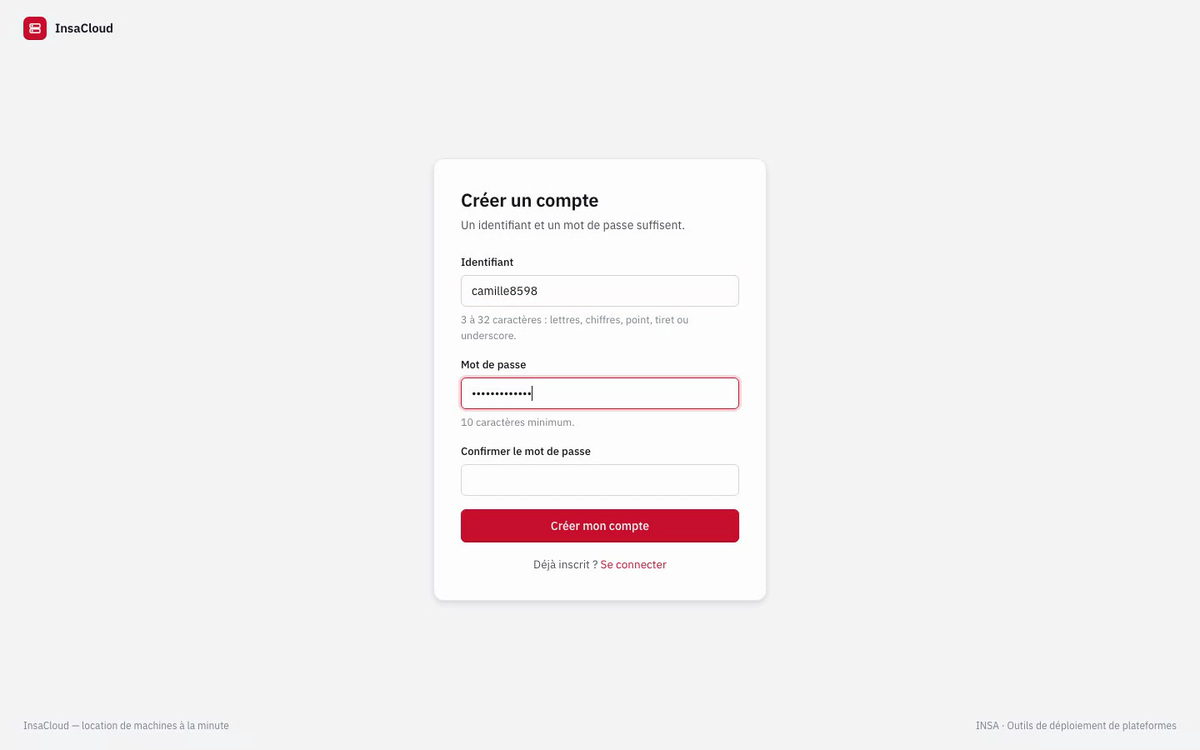
\includegraphics[width=\textwidth]{../docs/02-inscription.png}
\end{minipage}\hfill
\begin{minipage}{0.48\textwidth}
  \centering
  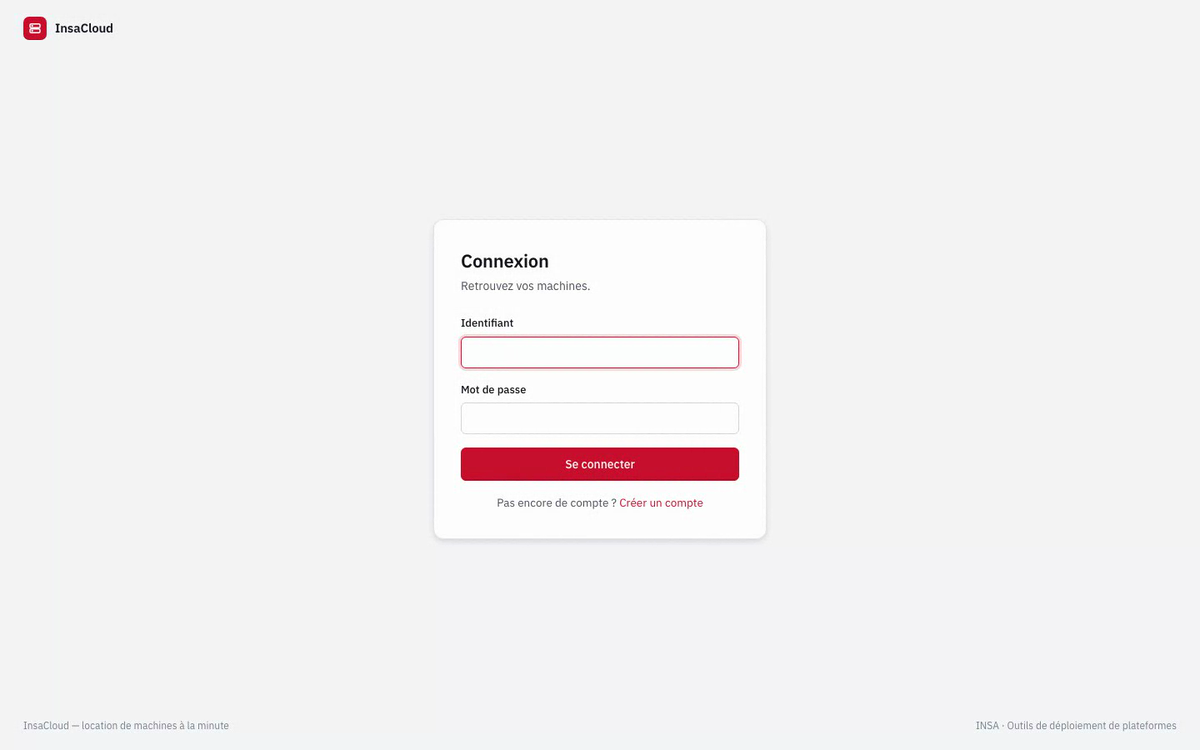
\includegraphics[width=\textwidth]{../docs/01-connexion.png}
\end{minipage}
\caption{Inscription et connexion. La politique de mot de passe est vérifiée
côté serveur : un contrôle fait uniquement dans le navigateur se contourne en
désactivant JavaScript.}
\end{figure}

\section{Empreinte et chiffrement, à ne pas confondre}

\begin{notion}{Deux besoins, deux mécanismes}
Le mot de passe d'un \emph{compte} est \textbf{haché} (\cmd{pbkdf2:sha256}) :
l'opération est à sens unique, on ne peut pas le retrouver, seulement vérifier
qu'un essai donne la même empreinte.

Le mot de passe \emph{root d'une machine louée} est \textbf{chiffré} : il doit
pouvoir être réaffiché, donc l'opération doit être réversible.

Hacher le second le rendrait inutilisable ; chiffrer le premier serait une
faute.
\end{notion}

Cinq échecs de connexion verrouillent temporairement le compte. Les tentatives
sont enregistrées avec l'adresse IP, dans une table indexée.

\section{Les en-têtes et la politique de contenu}

\begin{center}
\small
\begin{tabularx}{\textwidth}{@{}lX@{}}
\toprule
\textbf{En-tête} & \textbf{Effet} \\
\midrule
\cmd{Strict-Transport-Security} & le navigateur refuse ensuite le HTTP en clair \\
\cmd{X-Content-Type-Options} & interdit de deviner le type d'un fichier \\
\cmd{X-Frame-Options} & empêche l'inclusion du site dans un cadre \\
\cmd{Content-Security-Policy} & \cmd{default-src 'self'} : aucune ressource externe \\
\bottomrule
\end{tabularx}
\end{center}

\begin{retenir}
Une CSP stricte a un coût : plus de CDN, plus de script en ligne. Tailwind est
donc précompilé et les polices sont hébergées localement. C'est plus de travail
au départ, et cela supprime d'un coup toute une famille d'attaques par
injection de script.
\end{retenir}

\chapter{La haute disponibilité}
\label{chap:ha}

\section{Le scénario exact du cahier des charges}

L'énoncé décrit un test précis : éteindre un worker et vérifier que l'instance
repart ailleurs. Voici ce qui se passe, mesuré sur un cluster réel.

\begin{center}
\small
\begin{tabularx}{\textwidth}{@{}lX@{}}
\toprule
\textbf{Instant} & \textbf{Événement} \\
\midrule
T\,+\,0 s & \cmd{vagrant halt worker1} : l'agent cesse de battre \\
T\,+\,90 s & le Faucheur déclare \cmd{worker1} \cmd{OFFLINE} \\
T\,+\,90 s & la machine est recréée sur \cmd{worker2}, \cmd{migrations} passe à 1 \\
T\,+\,100 s & l'utilisateur voit un nouveau port et un nouveau mot de passe \\
plus tard & \cmd{worker1} redémarre, son agent se réinscrit en moins de 10 s \\
\bottomrule
\end{tabularx}
\end{center}

\begin{lstlisting}[language=Python,caption={\fichier{2\_webapp/services.py} --- la reprise}]
def recreer_ailleurs(instance: dict) -> Resultat:
    """
    Recree une instance sur un autre worker apres la panne du sien.

    Le conteneur est reconstruit a partir de la meme image, avec un mot de passe
    neuf — l'ancien vivait dans un conteneur devenu inaccessible. La location
    n'est pas touchee : l'utilisateur conserve la duree qu'il a payee.
    """
    ancien_noeud = instance["worker"]
    candidat = db.select_available_worker()
    if candidat is None or candidat["hostname"] == ancien_noeud:
        return Resultat.echec("Aucun worker de repli disponible.", code=503)
    ...
    db.move_instance(instance["id"], ports["container_id"], nouveau_noeud,
                     ports["port"], ports["term_port"], ports["gui_port"])
    db.set_instance_password(instance["id"], encrypt_secret(mot_de_passe))
\end{lstlisting}

Noter ce que ce code \emph{ne} fait pas : il ne touche pas à la table
\texttt{rentals}. C'est tout l'intérêt de la séparation du
chapitre~\ref{chap:modele}.

\section{Le compteur de migrations}

La colonne \cmd{migrations} de la table \texttt{instances} s'incrémente à
chaque reprise. Ce n'est pas décoratif : c'est la preuve observable qu'une
reprise a eu lieu, et c'est ce que vérifie le test d'intégration.

\begin{retenir}
Quand une fonctionnalité est difficile à observer, ajoutez-lui un compteur.
Sans \cmd{migrations}, il faudrait lire les journaux pour savoir si la reprise
a fonctionné --- et un test ne peut pas raisonnablement lire des journaux.
\end{retenir}

\chapter{Sauvegarder le travail avant destruction}
\label{chap:archives}

\section{Le besoin}

Détruire une machine détruit sa couche inscriptible. Un utilisateur qui a
travaillé trente minutes perd tout. Ce n'est demandé nulle part dans le cahier
des charges --- c'est un ajout, proposé par un contributeur extérieur et
intégré après correction.

\section{Le principe : un flux, pas un fichier temporaire}

\begin{lstlisting}[language=bash]
docker exec <conteneur> tar czf - -C / root home
\end{lstlisting}

Le tiret à la place du nom de fichier demande à \cmd{tar} d'écrire sur la
sortie standard. Python lit ce flux et l'écrit sur le disque du contrôleur. Pour
un worker distant, le transport SSH du client Docker fait passer le flux : rien
de plus n'est exposé sur le réseau, et rien n'est écrit dans le conteneur.

\begin{lstlisting}[language=Python,caption={\fichier{2\_webapp/archives.py} --- lire le flux sous contrainte}]
    # O_EXCL : on ne reecrit jamais un fichier existant. Mode 0600 des la
    # creation : l'archive peut contenir des cles ou des mots de passe.
    fd = os.open(destination, os.O_WRONLY | os.O_CREAT | os.O_EXCL, 0o600)
    with os.fdopen(fd, "wb") as sortie, subprocess.Popen(
            commande, stdout=subprocess.PIPE, stderr=subprocess.DEVNULL) as processus:

        def _delai():
            delai_depasse.set()
            processus.kill()

        minuteur = threading.Timer(ARCHIVE_TIMEOUT, _delai)
        minuteur.start()
        try:
            while bloc := processus.stdout.read(TAILLE_BLOC):
                taille += len(bloc)
                if taille > ARCHIVE_MAX_BYTES:
                    processus.kill()
                    return {"status": STATUS_TOO_LARGE}
                sortie.write(bloc)
                empreinte.update(bloc)
        finally:
            minuteur.cancel()
\end{lstlisting}

\begin{notion}{Pourquoi un minuteur et pas un test dans la boucle}
On pourrait vérifier le temps écoulé à chaque tour de boucle. Cela ne
marcherait pas : \cmd{read()} \emph{bloque} tant que Docker --- ou la connexion
SSH --- n'envoie rien. Si le nœud se fige, la boucle ne tourne plus du tout et
aucun test n'est évalué.

Un fil séparé qui tue le processus au bout du délai est la seule façon de
garantir la sortie.
\end{notion}

\section{La règle qui prime sur tout}

\begin{lstlisting}[language=Python,caption={\fichier{2\_webapp/archives.py} --- l'invariant du module}]
"""
Regle de conception : `archiver_conteneur` ne leve JAMAIS d'exception. Un
echec d'archivage (noeud injoignable, archive trop lourde, disque plein) doit
etre signale a l'appelant, pas l'empecher de detruire la machine : sinon une
machine expiree resterait en vie indefiniment.
"""
\end{lstlisting}

\begin{retenir}
Une fonctionnalité secondaire ne doit jamais pouvoir bloquer une fonctionnalité
essentielle. Ici, sauvegarder est un service rendu ; détruire à l'échéance est
une obligation. Si l'un doit céder, ce n'est pas le second.
\end{retenir}

\section{Retenter sans boucler}

La première version ne retentait jamais un archivage raté : une simple coupure
SSH condamnait les fichiers. Mais retenter à chaque cycle du Faucheur serait
pire : sur un nœud durablement muet, chaque passage attendrait le délai maximal
de 45 secondes, toutes les 10 secondes.

\begin{lstlisting}[language=Python,caption={\fichier{2\_webapp/database.py} --- le compromis}]
def archivage_deja_fait(instance_id: int, delai_avant_reprise: int = 600) -> bool:
    """
    Une archive reussie n'est jamais refaite : la destruction peut etre
    retentee pendant plusieurs cycles du Faucheur, le travail n'est copie
    qu'une fois.

    Un echec, en revanche, vient parfois d'un incident passager — un noeud
    brievement injoignable. On retente alors, mais pas a chaque cycle.
    """
\end{lstlisting}

\begin{notion}{Le téléchargement, et ses trois protections}
Une archive contient les fichiers privés d'un utilisateur. La route de
téléchargement les protège de trois façons :
\begin{enumerate}
\item le propriétaire est vérifié \emph{dans la requête SQL} : l'archive d'un
  autre compte répond 404, exactement comme une archive inexistante --- cela ne
  révèle rien sur les comptes voisins ;
\item \cmd{send\_from\_directory} joint le chemin au dossier des archives et
  refuse toute sortie (\cmd{../}), même si la base était altérée ;
\item la réponse est un téléchargement (\cmd{attachment}), jamais affichée
  dans la page.
\end{enumerate}
\end{notion}
